
\subsection{Tasks Correctness}
\label{cp6:correctness}



When assisted by a tool able to automatically highlight text identified as relevant to a task, we expect that a developer can produce a solution 
that is equally or more correct than the solution of a developer who attempted a task without tool support. 


To compute how correct a participant's solution is, 
we compile their code and run it against a set of 10 test cases that check whether it produces the correct output for each given test input. 
Hence, \textit{correctness} represents the number of passing test cases of a solution (Equation~\ref{eq:cp6-correctness}).
For example, if the solution of a participant passes 7 out of 10 test cases, we would assign a 
correctness score of $7$ to this solution. 
A solution with compile errors has a correctness score of $0$.


\smallskip
\begin{small}


\begin{equation}
    Correctness = \text{\textit{\# of passing test cases}}
    \label{eq:cp6-correctness}
\end{equation}
\end{small}

% \subsubsection{Results}



\begin{figure}[h!]
    \centering
    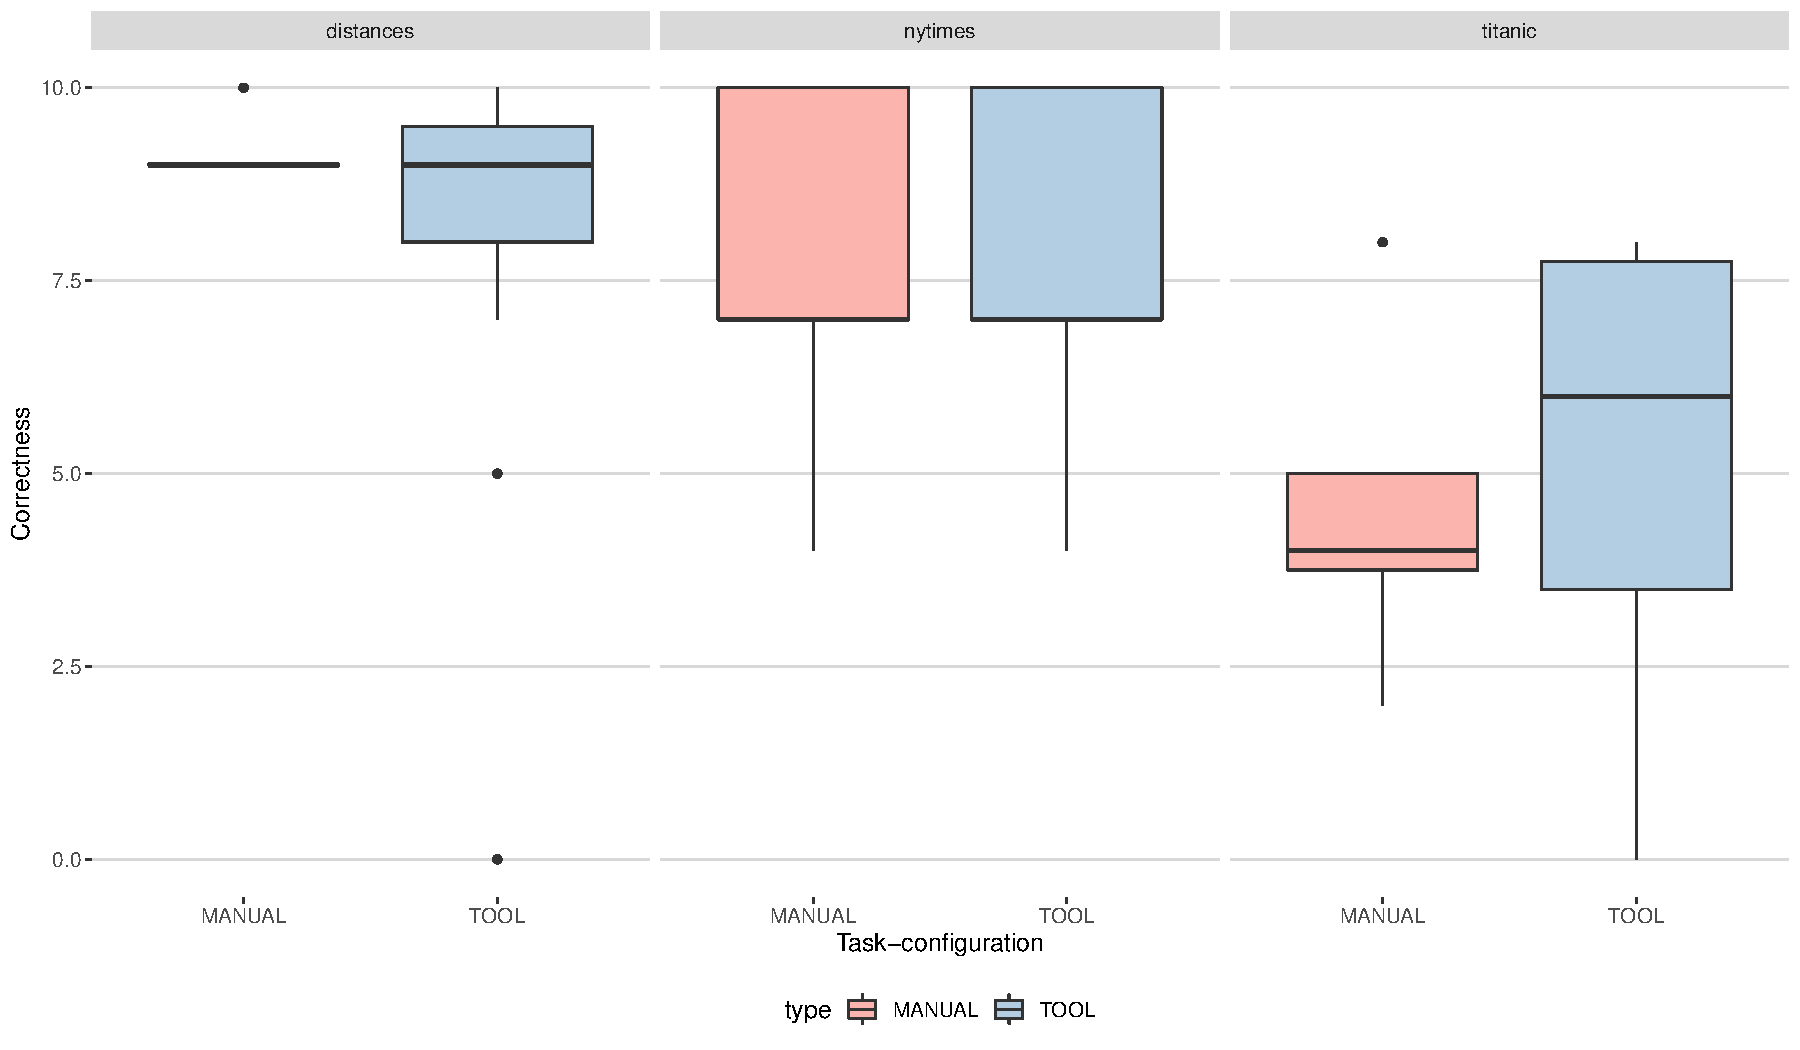
\includegraphics[width=\textwidth]{cp6/correctness_overall.pdf}
    \caption{Boxplot comparing how correct are the solutions of each task done with and without tool support}
    \label{fig:correctness-by-task}
\end{figure}

